% !TEX TS-program = XeLaTeX
\documentclass{ISCISC2020}

% تقریبا تمامی بسته‌های مورد نیاز برای یک مقاله در استایل فراخوانی شده است. اما در هر صورت در صورتی‌که می‌خواهید بسته‌ای را فراخوانی کنید به صورت زیر عمل کنید. مثلا ما در کد زیر دوبسته glossaries و tikz را فراخوانی کرده‌ایم.
\makeatletter
\bidi@BeforePackage{xepersian}{
% \RequirePackage{tikz}
% \RequirePackage{glossaries}
\RequirePackage{natbib}
}
\makeatother


% عنوان مقاله را در این قسمت وارد کنید. 
\title{
Pretender :Defender هنگامی که به روزرسانی های Defender Windows تبدیل به یک خطر امنیتی می شود
}
\date{}
% اسامی نویسندگان و همچنین اطلاعات مربوط به آن‌ها را در این قسمت وارد کنید. 
\author[1]{محمدحسین عباسپور ۹۹۵۲۱۴۳۳}
\author[1]{فرزان رحمانی ۹۹۵۲۱۲۷۲}
\author[2]{ابوالفضل دیانت}

\affil[1]{
دانشجوی کارشناسی مهندسی کامپیوتر، دانشگاه علم و صنعت ایران، تهران،
آدرس پست الکترونیکی:m\_abbaspoor80@comp.iust.ac.ir
}
\affil[1]{

دانشجوی کارشناسی مهندسی کامپیوتر، دانشگاه علم و صنعت ایران، تهران، 
آدرس پست الکترونیکی: farzan\_rahmani@comp.iust.ac.ir
}
\affil[2]{
استادیار دانشکده مهندسی کامپیوتر، دانشگاه علم و صنعت ایران، تهران، آدرس پست الکترونیکی: adiyanat@iust.ac.ir
}

\begin{document}
\maketitle

\begin{abstract}
این مقاله یک آسیب‌پذیری جدید کشف شده در فرآیند به‌روزرسانی Windows Defender را توصیف می‌کند. این آسیب‌پذیری به یک مهاجم غیرمجاز اجازه می‌دهد تا کنترل Windows Defender را به دست آورده و رفتار آن را برای اهداف مخرب دستکاری کند. این حمله ضعفی را در روشی که Windows Defender به‌روزرسانی‌های امضا، به‌ویژه فایل‌های Base VDM و VDM Delta را تأیید می‌کند، ایجاد می‌کند. ما سه بردار حمله را نشان می‌دهیم: حذف امضاهای تهدید، دستکاری لیست مجاز FriendlyFiles و راه‌اندازی یک حمله انکار سرویس. تحقیقات ما اهمیت ارزیابی مداوم نرم افزارهای امنیتی و پیاده سازی مکانیزم های اعتبارسنجی به روز رسانی قوی را برجسته می کند.
% (\lr{Style}) برای کلمات انگلیسی  

\end{abstract}

\begin{keywords}
آسیب پذیری\LTRfootnote{Vulnerability}،
 \lr{Windows Defender}،
 به‌روزرسانی امضا\LTRfootnote{Signature Update}،
 بردار حمله\LTRfootnote{Attack Vector}،
 انکار سرویس\LTRfootnote{Denial-of-Service}،
 افزایش امتیاز محلی\LTRfootnote{Local Privilege Escalation}.
\end{keywords}

\section{پیش زمینه}
 Labs SafeBreach \lr{[1]}
 تحقیقات امنیت سایبری پیشرفته را بر اساس بینش های دنیای واقعی و مشاهدات حملات «در 
طبیعت» ارائه می‌کند. در 
سال، 2012 محققان آزمایشگاه کسپرسکی بدافزار Flame\lr{[2]} را کشف کردند که عوامل تهدید تحت حمایت دولت از آن 
برای سوء استفاده از فرآیند به روزرسانی ویندوز با استفاده از حملات MITM پیچیده استفاده می کردند. آنها توانستند با 
موفقیت فرآیند به روزرسانی ویندوز را ربوده و درخواست های به روزرسانی را از رایانه های آلوده به سرورهای خود 
هدایت کنند. سپس آنها توانستند به روزرسانی های مخرب را ارائه کنند و از این دسترسی برای حفظ پایداری 
دستگاه های آسیب دیده استفاده کنند.


ما تعجب کردیم که آیا می توان به طور مشابه فرآیند به روز رسانی Defender Windows را ربود و به طور 
بالقوه محصول Defender Windows را برای کنترل آن برای اهداف مخرب بیشتر نقض کرد. ما همچنین می خواستیم 
بدون اجرای حملات پیچیده، MITM بدون گواهی جعلی و به عنوان یک کاربر غیرمجاز، این کار را انجام دهیم.

\section{فرآیند تحقیق}
\subsection{آشنایی با فرآیند آپدیت ویندوز دیفندر}
برای تعیین بهترین مسیر اقدام، اولین قدم ما درک جامع فرآیند به روزرسانی Defender Windows بود. متوجه شدیم کهDefender Windows به طور دوره ای به مرکز به روزرسانی مایکروسافت پینگ می کند و هرگونه به روزرسانی جدید 
تعریف امضا را بررسی می کند. اگر یک به روزرسانی در دسترس باشد، معمولا ًبه صورت یک فایل اجرایی به نام   End Front Antimalware Protection Microsoft (MPAM-FE) بازگردانده می شود.

\begin{figure}[h]
	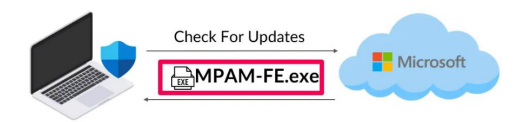
\includegraphics[width=\linewidth]{Images/1.png}
 	\caption{روند End Front Antimalware Protection Microsoft}

\end{figure}

پس از دانلود و تجزیه و تحلیل فایل MPAM، متوجه شدیم که شامل یک فایل کابینت (CAB) است که شامل دو فایل 
اجرایی- dll[.]mpengine و exe[.]MpSigStub، و چهار فایل با پسوند VDM است. پس از اجرای فایل MPAM، 
متوجه شدیم که فایل MpSigStub را نیز به عنوان یک فرآیند فرزند برای دانلود به روزرسانی ها اجرا می کند. 


مادر ابتدا چیز زیادی در مورد فایل های VDM نمی دانستیم اما به زودی اهمیت آنها را در تحقیقات خود کشف کردیم. 
فایلهای VDM فایل های قابل حمل قابل اجرا هستند. با این حال، آنها را نمی توان اجرا کرد زیرا هیچ منطق کدی 
ندارند.ما در ابتدا فرض می کردیم که آنها فایل های داده خاصی هستند که حاوی امضاهای تشخیص هستند. ما 
مشاهده کردیم که دو نوع فایل VDM وجود دارد: Base و Delta، با تفاوت اصلی در اندازه آنها. پس از مطالعه جزئیات 
بیشتر هر فایل، توانستیم بفهمیم که چگونه فایل های Base و VDM Delta برای ارسال به روزرسانی های جدید پایگاه 
داده امضا به Defender Windows استفاده می شوند. ما همچنین متوجه شدیم که مایکروسافت تمام فایل های 
موجوددر فایل CAB را به صورت دیجیتال امضا کرده است تا از دستکاری در فرآیند به روزرسانی جلوگیری کند.

\begin{figure}[h]
	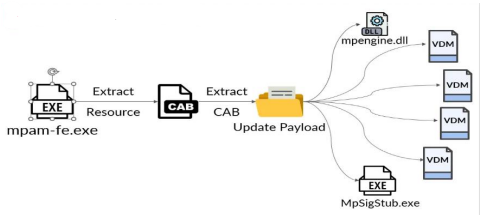
\includegraphics[width=\linewidth]{Images/2.png}
	\caption{منابع mpam-fe.exe}
\end{figure}

%\begin{figure*}[t]
\begin{figure}[h]
	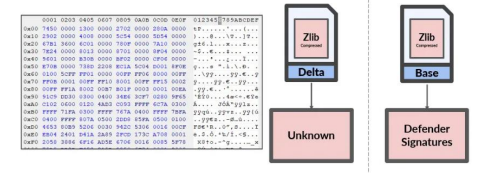
\includegraphics[width=\linewidth]{Images/4.png}
	\caption{فایل دلتا پیچیده تر است و نیاز به تجزیه و تحلیل بیشتری دارد.}
\end{figure}
%\end{figure*}

\subsection{انتخاب فایل مناسب برای سازش}
ماابتدا تصمیم گرفتیم dll[.]mpengine را با فایل dll[.]mpengine جعلی خود جایگزین کنیم به این امید که 
Defender کنترل آن را به ما واگذار کند. وقتی سعی کردیم فرآیند به روزرسانی را اجرا کنیم، شکست خورد زیرا 
Defender تشخیص داد که dll[.]mpengine توسط مایکروسافت امضا نشده است و نمی تواند به روزرسانی را اجرا 
کند.

\begin{figure}[h]
	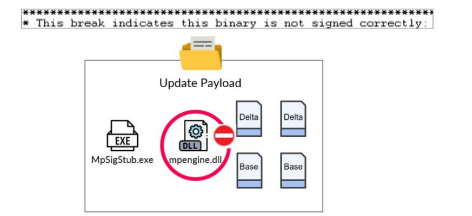
\includegraphics[width=\linewidth]{Images/3.png}
	\caption{دستکاری فایل VDM}
\end{figure}

بعد،تصمیم گرفتیم توجه خود را به فایل های VDM معطوف کنیم. ما در ابتدا زمانی به موفقیت هایی دست یافتیم که 
توانستیم یک فایل VDM قدیمی (بدون تغییر هیچ یک از داده ها) را به روز کنیم و Defender را باور کنیم که نسخه 
جدیدی از آن فایل است. این اولین سرنخ ما را به ما داد که در مسیر درستی هستیم.


سپس ما سعی کردیم یک بایت تصادفی را در فایل Delta VDM تغییر دهیم و آن را به عنوان یک به روز رسانی فشار 
دهیم،اما این روش موفق نشد. واضح است که ما چیزی را در روند فکر خود گم کرده بودیم. ما همچنین در تعجب 
ماندیم که چگونه می توانیم به عنوان یک کاربر غیرمجاز به همه اینها دست پیدا کنیم. پاسخ در تجزیه و تحلیل فایل به روز 
رسانی امضای حفاظت از بدافزار (MpSigStub) بود، که نشان داد هدف واقعی فایل VDM ارائه به روزرسانی های 
امضای بدافزار به Defender Windows است.

\subsection{آشنایی با فایل های VDM}
فایل هایVDM فایل های اجرایی قابل حمل ویندوز هستند که شامل یک بخش منبع با داده های فشرده است که 
شامل امضاهای Defender است. امضاها در هر دو فایل Base و VDM Delta فشرده شده اند، اما در کمال تعجب، 
رمزگذاری نشده اند. پس از فشرده سازی امضاها در فایل Base، به راحتی می توانیم شروع و پایان امضاها و رشته 
بدافزار واقعی را با نام های بدافزار به وضوح در رشته مشخص کنیم. ما توانستیم مطمئن شویم که این فایل اصلی 
استکه Defender برای امضای بدافزار بررسی کرده است. فایل دلتا به طور قابل توجهی پیچیده تر بود و نیاز به تجزیه 
وتحلیل عمیق تری دارد.


%\begin{figure}[h]
	%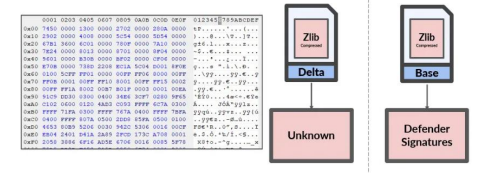
\includegraphics[width=\linewidth]{Images/4.png}
%\end{figure}

\subsection{درک ساختار امضا}
ما فرض کردیم که فایل Base شامل اکثر منطق امضایی است که در قالبی قابل فهم ارائه شده است. با تجزیه و 
تحلیل بیشتر امضاهای فایل پایه، ما توانستیم تعیین کنیم که هر تهدید با امضای نوع C5 شروع شده است. تهدید 
مجموعه ای از امضاها است. این امضاها رشته ها یا توالی بایت های منحصر به فردی هستند که به خانواده بدافزارها 
تعلق دارند. مجموعه امضاها همیشه با Signature End\_Threat (یک نوع 5 بعدی) به پایان می رسد.


فایلBase در واقع دنباله ای از تهدیدات است – وقتی یک تهدید تمام می شود، تهدید بعدی شروع می شود و غیره. با 
استفاده از فرمت امضا، توانستیم بیش از دو و نیم میلیون امضا را از فایل Base استخراج کنیم. با در دست داشتن این 
اطلاعات،ما سعی کردیم نام تهدید مرتبط با یک امضای خاص را تغییر دهیم و فایل VDM را مجددا ًفشرده کردیم به این 
امیدکه Defender این به روزرسانی را بپذیرد. ما سعی کردیم با فایل Base بیشتر سرهم بندی کنیم و حتی سعی کردیم 
مقدارچک افزونگی چرخه ای (CRC) را دستکاری کنیم به این امید که Defender بالاخره این تغییر را بپذیرد. اما این 
تلاش نیز شکست خورد.


آن موقع بود که متوجه شدیم نمی توانیم فایل دلتا را نادیده بگیریم. ما قبلاً رابطه بین فایل های Base و VDM Delta را 
اشتباه متوجه شده بودیم. دو جفت VDM وجود دارد: جفت اول شامل تعاریف ضد ویروس Defender و جفت دوم 
شامل تعاریف نرم افزارهای جاسوسی است. هر یک از این جفت ها از نظر فرمت امضا و پرونده یکسان هستند. در 
طول به روز رسانی، هر دو فایل Base و Delta درگیر می شوند. ادغام فایل Base را می گیرد و Delta به سادگی 
تغییراتی را که باید در این فایل Base ایجاد شود را تعریف می کند. فایل خروجی به دست آمده نشان دهنده نسخه به 
روزشده از دلتا خواهد بود. ما متوجه شدیم که برای اصلاح امضاهای پایه، باید یک فایل دلتا ارائه کنیم که دقیقا ًپایگاه 
رابا تغییرات مورد نظر اصلاح کند.
%\begin{figure*}[t]
\begin{figure}[h]
	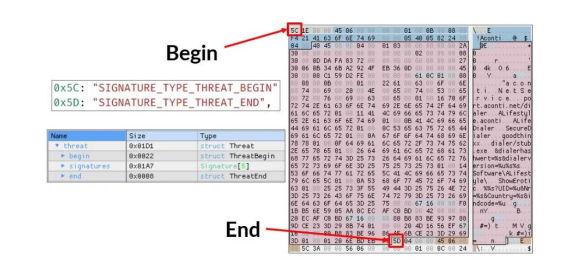
\includegraphics[width=\linewidth]{Images/5.png}
	\caption{داخل یک فایل VDM}
\end{figure}
%\end{figure*}

\subsection{درک فرآیند ادغام و اعتبارسنجی کلی}
فایل دلتا یک فایل مبتنی بر امضا است. همیشه شامل دو امضا است که نوع دوم یک شیء بزرگ باینری (BLOB)
است.اعتبار سنجی اول به سادگی بررسی می کند که آیا ZlibCompressedData فایل دلتا با مقایسه مقدار CRC
موردانتظار در ZlibDataHeader با CRC محاسبه شده در ZlibCompressedData تغییر نکرده است.


تجزیه و تحلیل بیشتر همچنین نقطه دقیقی را که Defender اقدامات مختلف را تجزیه و تحلیل می کند نشان داد. ما 
دونوع اقدام را شناسایی کردیم: CopyFromDelta و CopyFromDelta .CopyFromBase برای کپی کردن بایت های 
<size> از دلتا در ادغام استفاده می شود. CopyFromBase برای کپی کردن بایت های <size> از یک <offset> در 
Base در ادغام استفاده می شود. ما یک اسکریپت برای ادغام داده ها بین فایل Base و فایل Delta نوشتیم. ما 
همچنین توانستیم دو عددی را که Defender برای اهداف اعتبارسنجی استفاده می کند شناسایی کنیم: MergeSize و 
.MergeCRC32


پساز درک کل فرآیند ادغام، امضا و اعتبارسنجی، می خواستیم دانش خود را آزمایش کنیم و بررسی کنیم که آیا در 
ارائه به روزرسانی جعلی به Defender Windows موفق خواهیم بود یا خیر. موفقیت آمیز بود و ما توانستیم 
Defender را با یک پایگاه داده جعلی و بدون امضا با استفاده از یک کاربر غیرمجاز به روز کنیم.



\section{استفاده از Defender Windows}
پس از درک کامل فرآیند به روزرسانی Defender و تعیین بهترین راه برای جعل به روزرسانی و کنترل Defender، 
تصمیم گرفتیم قابلیت آسیب پذیری خود را به روش های جداگانه تأیید کنیم. به منظور اعتبارسنجی و پشتیبانی از همه 
بردارهای حمله خود، یک ابزار کاملا ًخودکار به نام pretender-wd مخفف Pretender Defender Windows ایجاد 
کردیم.

\subsection{بردار حمله ۱ - حذف تهدیدات LaZagne}
همانطورکه در بالا اشاره کردیم، امضاهای Defender Windows نتیجه ترکیب داده های فایل های Base و Delta
هستند.این داده های ترکیبی هر تهدید را با نام آن شناسایی می کند، که به محققان اجازه می دهد هدف آن را شناسایی 
کنند.می خواستیم ببینیم که آیا امکان حذف یک تهدید از پایگاه داده امضای Defender Windows وجود دارد یا خیر. 
برای این منظور، ما سعی کردیم تمام تهدیداتی را که حاوی کلمه LaZagne در نام آنها بودند حذف کنیم.


LaZagne راشناسایی نکرد، زیرا امضای آن با هیچ چیز در پایگاه داده آن مطابقت نداشت ابزار مخرب Defender
Windows .را دانلود و اجرا کنیم. این بار موفقیت آمیز بود LaZagne را در پایگاه داده امضای خود نداشت. پس از 
تکمیل آپدیت، سعی کردیم دوباره ابزار LaZagne به روزرسانی جعلی را ارائه کردیم که عبارت ،pretender-wd
بلافاصله آن را با نام شناسایی کرد و اجرای آن را متوقف کرد. با استفاده از ابزار Defender ،را به عنوان یک کاربر 
غیرمجازدانلود و اجرا کنیم LaZagne یک برنامه منبع باز است که برای بازیابی تعداد زیادی رمز عبور ذخیره شده در 
رایانه محلی استفاده می شود.

\subsection{بردار حمله ۲ - FriendlyFiles}
سپس توجه خود را به ویژگی به نام FriendlyFiles معطوف کردیم که اساسا ًیک لیست مجاز در Defender
Windows است. FriendlyFiles به Defender Windows اجازه می دهد تا بداند کدام فایل های اجرایی باید بر 
اساس مقدار الگوریتم هش ایمن خود (SHA) عمل کنند. تجزیه نوع امضای FriendlyFile لیست بسیار طولانی و 
مرتب شده ای از هش ها را نشان داد. در این میان ما شناسایی کردیم. یکهش متعلق به کتابخانه زمان اجرا جعبه مجازی Oracle. می خواستیم بدانیم اگر هش این فایل را با مقدار هش 
شناخته شده Mimikatz جایگزین کنیم، چه اتفاقی می افتد.


وقتی برای اولین بار سعی کردیم Mimikatz را دانلود کنیم، Defender Windows بلافاصله ما را متوقف کرد. سپس از 
ابزارpretender-wd خود استفاده کردیم تا هش FriendlyFile را با هش Mimikatz جایگزین کنیم و از طریق یک 
به روزرسانی جعلی به Defender Windows این کار را انجام دهیم. پس از آپدیت، سعی کردیم Mimikatz را دانلود 
کرده و دوباره اجرا کنیم. ما نه تنها در نصب Mimikatz موفق بودیم، بلکه توانستیم تمام اعتبارهای ذخیره شده را از آن 
دستگاه استخراج کنیم.

\subsection{بردار حمله ۳ - انکار سرویس}
سومین و آخرین بردار حمله ای که ما اعتبارسنجی کردیم، انکار سرویس (DOS) بود. ما تصمیم گرفتیم که Defender
Windows همه فایل های قابل حمل قابل حمل (PE) را با تغییر امضای Emotet برای گنجاندن «رشته Stub Mode
Dos «که در هر فایل PE به عنوان یک امضای مخرب جدید ظاهر می شود، حذف کند. اگر Defender در فایل های 
مختلف سیستم عامل (OS) با رشته «!این برنامه در حالت dos اجرا نمی شود» برخورد می کرد، به طور خودکار آنها را 
حذف می کرد.


مااز pretender-wd استفاده کردیم تا اجازه دهیم «رشته Stub Mode Dos «با رشته ما با امضای مخرب Emotet
اصلاح و به روز شود. به محض اینکه Defender متوجه این موضوع شد، بلافاصله به ما در مورد آن هشدار داد. 
همچنینDefender کل پوشه درایور رایانه شخصی را اسکن کرد و چندین فایل حیاتی ویندوز را با امضای مخرب 
یکسان شناسایی کرد و بلافاصله آنها را حذف کرد. ما سعی کردیم رایانه شخصی را مجدداً راه اندازی کنیم، اما 
نتوانستیم،و منجر به انکار دائمی سرویس شد.

\subsection{بردار حمله احتمالی آینده - امکان دستیابی به افزایش امتیاز محلی}
ما یک بردار حمله احتمالی آینده را شناسایی کرده ایم که می تواند منجر به افزایش امتیاز محلی شود. در طول تحقیق ما 
همچنین متوجه شدیم که فایل امضا حاوی 30 هزار اسکریپت در زبان برنامه نویسی LUA است. مایکروسافت از یک 
هدرLUA اصلاح شده استفاده می کند، اما ما توانستیم آن را دیکامپایل کرده و کد منبع همه اسکریپت های K30 LUA
رااستخراج کنیم. با دسترسی به کل کد منبع، به طور بالقوه می توانیم کد اجرا شده را با کد اصلاح شده خود جایگزین 
کنیم و شاید به افزایش امتیاز محلی (LPE) برسیم.

\section{پاسخ فروشنده}
به محض اینکه مایکروسافت را از کشف آسیب پذیری خود مطلع کردیم-2023-24934،CVE، آنها آن را تایید کردند، 
اقدام فوری انجام دادند و وصله ای منتشر کردند که امضای دیجیتال همه فایل های VDM را تایید می کند. نسخه ثابت  Platform Protection Malware Microsoft نسخه ۴.۱۸.۲۳۰۳.۸ است.

\section{نکات کلیدی}
بر اساس یافته های مرتبط با این تحقیق، ما معتقدیم درک این نکات مهم است:
\begin{itemize}
\item
اگر دشمنان انگیزه کافی داشته باشند، حتی مطمئن ترین کنترل های امنیتی نیز ممکن است مستعد دور زدن آن ها باشند. قبل از اینکه مهاجم بتواند از آنها سوء استفاده کند، امنیت این کنترل ها باید به صورت دوره ای آزمایش و رفع شود.
\item
استفاده از فایل های امضا شده دیجیتال همیشه به معنای افزایش امنیت نیست. وظیفه فروشنده امنیتی است که اطمینان حاصل کند که مهاجم نمی تواند از فرآیندهای داخلی سوء استفاده کند و آنها را به نفع خود خراب کند.
\item
بر اساس پتانسیل فرآیند به روز رسانی امضای بدافزار به عنوان یک بردار حمله جدید، تحقیقات بیشتری برای اطمینان از امنیت این فرآیند مورد نیاز است.
\end{itemize}

\section{نتیجه گیری‌}
این تحقیق یک آسیب‌پذیری مهم در فرآیند به‌روزرسانی Windows Defender را برجسته می‌کند. این امر بر اهمیت ارزیابی مداوم نرم افزار امنیتی و مکانیسم های اعتبارسنجی به روز رسانی قوی تاکید می کند. توصیه می کنیم هوشیار بمانید و آخرین وصله های امنیتی را برای کاهش چنین خطراتی اجرا کنید.


به علاوه، پیامدهای تحقیق ما قابل توجه است، زیرا Defender Windows ابزار بسیار شناخته شده و قابل اعتمادی است که 
بسیاری از سازمان ها از آن به عنوان اولین خط دفاعی استفاده می کنند. برای کمک به کاهش تأثیر بالقوه این 
آسیب پذیری ها،ما داریم:
\begin{itemize}
\item
با مسئولیت پذیری یافته های تحقیقاتی خود را به مایکروسافت فاش کرد و آنها برای آسیب پذیری کشف 
شده ما (\lr{CVE-2023-24934})\lr{[3]} راه‌حلی صادر کردند.
\item
شامل ابزارهایی است که تأیید این آسیب پذیری را امکان پذیر می کند و به عنوان پایه ای برای 
تحقیقات بیشتر و توسعه بردارهای حمله جدید عمل می کند.
\item
تحقیقات خود را در اینجا و اخیراً با جامعه امنیتی گسترده تر به اشتراک گذاشتیم کلاه سیاه\lr{[4]} ارائه به این 
امیدکه کاربران هوشیار بمانند و درک کنند که حتی مطمئن ترین ابزارهای امنیتی نیز می توانند توسط 
یک مهاجم با انگیزه به خطر بیفتند.
\end{itemize}

\section*{سپاس‌گزاری}
از خداوند متعال بسيار سپاسگزاریم بابت توانی كه به مـا جهـت نوشـتن ايـن
مقاله اعطاء نمود. از جناب دكتر دیانت كه استاد ما در تهيه اين مقاله بوده‌اند
نيز بسيار تشكر ميكنیم. همچنين از خـانواده عزيـزمان كـه پشـتيبان و موجـب
دلگرمی ما هستند بينهايت سپاسگزاریم. 

% \bibliography{lib}
\section*{مراجع}

\begin{flushleft}
\lr{[1] SafeBreach Labs. Windows Defender Security Risk: Defender Pretender. https://www.safebreach.com/blog/defender-pretender-when-windows-defender-updates-become-a-security-risk/}
\newline
\lr{[2] Wired. Flame: Kaspersky Lab Uncovers a Super-Sophisticated Cyber Weapon. https://www.wired.com/2012/05/flame/}
\newline
\lr{[3] National Vulnerability Database (NVD). CVE-2023-24934. https://nvd.nist.gov/vuln/detail/CVE-2023-24934}
\newline
\lr{[4] Black Hat. Black Hat USA 2023 Briefings Schedule. https://www.blackhat.com/us-23/briefings/schedule/\#defender-pretender-when-windows-defender-updates-become-a-security-risk-32706}
\end{flushleft}

\theendnotes
\end{document}


